\documentclass[12pt]{article}
\pagenumbering{gobble}

\usepackage{amsmath}
\usepackage{amsfonts}
\usepackage{amssymb}
\usepackage{fancyhdr}
\usepackage[headheight=0.25in,margin=1in]{geometry}

\usepackage{tikz}
\usetikzlibrary{arrows.meta}

\newcommand{\parens}[1]{\left( #1 \right)}

\newcommand{\N}{\mathbb{N}}
\newcommand{\Z}{\mathbb{Z}}
\newcommand{\Q}{\mathbb{Q}}
\newcommand{\R}{\mathbb{R}}
\newcommand{\C}{\mathbb{C}}

\newcommand{\solution}{\textbf{Solution:}}
\newcommand{\proof}{\textbf{Proof:}}
\newcommand{\done}{\ensuremath{
    \strut\hfill\blacksquare
}}

\linespread{1.25}

\begin{document}
    \pagestyle{fancy}

    \fancyhead[L]{Computer Networks}
    \fancyhead[C]{Lab 3 - TCP}
    \fancyhead[R]{Alex Agruso}

    \begin{itemize}
        \item [Step 3.)] Packet \#5 from \verb|trace-tcp.pcap|:
        \begin{center}
            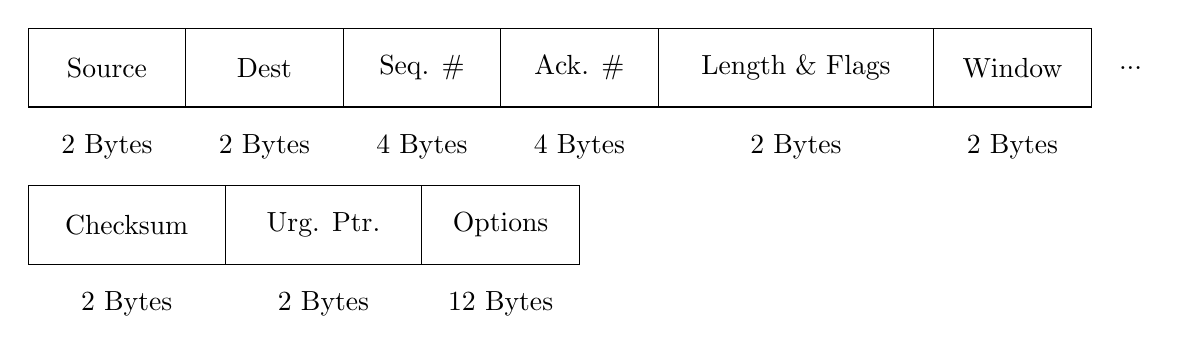
\begin{tikzpicture}
                \draw[] (0,0) rectangle (13.5,1);

                \draw[] (0,0) rectangle (2,1)
                node[midway] {Source};
                \node[] at (1,-0.5) {2 Bytes};

                \draw[] (2,0) rectangle (4,1)
                node[midway] {Dest};
                \node[] at (3,-0.5) {2 Bytes};

                \draw[] (4,0) rectangle (6,1)
                node[midway] {Seq. \#};
                \node[] at (5,-0.5) {4 Bytes};

                \draw[] (6,0) rectangle (8,1)
                node[midway] {Ack. \#};
                \node[] at (7,-0.5) {4 Bytes};

                \draw[] (8,0) rectangle (11.5,1)
                node[midway] {Length \& Flags};
                \node[] at (9.75,-0.5) {2 Bytes};

                \draw[] (11.5,0) rectangle (13.5,1)
                node[midway] {Window};
                \node[] at (12.5,-0.5) {2 Bytes};

                \draw[] (0,-1) rectangle (7,-2);

                \draw[] (0,-1) rectangle (2.5,-2)
                node[midway] {Checksum};
                \node[] at (1.25,-2.5) {2 Bytes};

                \draw[] (2.5,-1) rectangle (5,-2)
                node[midway] {Urg. Ptr.};
                \node[] at (3.75,-2.5) {2 Bytes};

                \draw[] (5,-1) rectangle (7,-2)
                node[midway] {Options};
                \node[] at (6,-2.5) {12 Bytes};

                \node[] at (14,0.5) {...};
            \end{tikzpicture}
        \end{center}

        \item [Step 4.)] Three-way Handshake:
        \begin{center}
            \begin{tikzpicture}[xscale=1.5]
                \node at (0,0) {Local};
                \draw[->] (0,-0.5) -- (0,-8);

                \node at (5,0) {Remote};
                \draw[->] (5,-0.5) -- (5,-8);

                \node[align=right] at (-0.5,-1.5) {0ms\\Seq: 0\\Ack: 0};

                \draw[->] (0,-1.5) -- (4.9, -3);
                \node[align=left] at (5.5,-3) {88ms\\Seq: 0\\Ack: 1};

                \draw[->] (5,-3.1) -- (0.1,-4.5);
                \node[align=right] at (-0.5,-4.5) {88ms\\Seq: 1\\Ack: 1};

                \draw[->] (0,-4.6) -- (4.9, -6);
                \node[align=left] at (5.85,-6) {88ms\\Seq: 1\\Ack: 1\\HTTP GET};
            \end{tikzpicture}
        \end{center}
        The round trip time for this instance was 88ms.

        \item [Step 4.1)] The options contained in the SYN packets were:

        \verb|Maximum Segment Size: 1046 bytes|

        \verb|Window scale: 3|

        \verb|Timestamps: TSval 256679793, TSecr 0|

        \verb|SACK permitted|

        The rest were NOP's or end-of-list indicators.

        \pagebreak
        \item [Step 4.2)] Connection teardown:
        \begin{center}
            \begin{tikzpicture}[xscale=1.5]
                \node at (0,0) {Local};
                \draw[->] (0,-0.5) -- (0,-8);

                \node at (5,0) {Remote};
                \draw[->] (5,-0.5) -- (5,-8);

                \node[align=right] at (-0.95,-1.5) {4111ms\\Seq: 192\\Ack: 1056771};

                \draw[->] (0,-1.5) -- (4.9, -3);
                \node[align=left] at (6,-3) {4198ms\\Seq: 1056772\\Ack: 193};

                \draw[->] (5,-3.1) -- (0.1,-4.5);
                \node[align=right] at (-0.95,-4.5) {4198ms\\Seq: 193\\Ack: 1056772};
            \end{tikzpicture}
        \end{center}
        The round trip time for this instance was 87ms, which is very close to the
        connection setup time.

    \item [Step 5.1)] Between 1 and 4 seconds, the download rate maintains
        a rough average of 30 packets/second, or 30,000 bytes/second.

    \item [Step 5.2)] Studying the trace, we find a common pattern of 2
        large packets with length 1434, then one much smaller packet with length 66.
        The larger packets tend to have a payload size of 1368 bytes, thus
        the approximate percentage of the download rate that contains actual content
        is given by:
        \[
            \frac{\text{payload size}}{\text{total packets size}}
            = \frac{2\times1368}{2\times1434 + 66}
            \approx 93\%
        \]

    \item [Step 5.3)] We can similarly find the approximate percentage of the download
        rate that contains ACK overhead:
        \[
            \frac{\text{ACK size}}{\text{total packets size}}
            = \frac{66}{2\times1434 + 66}
            \approx 2\%
        \]

    \item [Step 5.4)] Studying the trace, we find that subsequent Seq and Ack numbers match
        eachother the majority of the time.
    \end{itemize}
\end{document}
